%\documentclass[a4paper]{article}
%\usepackage{beamerarticle}

\documentclass[ignorenonframetext]{beamer}
\usepackage{beamerthemesplit}
\usepackage{amssymb}
\usepackage{verbatim}


\usepackage{../fhnw-beamer}

%\mode<article>{\usepackage{fullpage}}
%\mode<presentation>{\usetheme{Berlin}}

\date{\today}
\author{rolf.schmutz@fhnw.ch}
\institute{FHNW}
\title{Netzwerke und Kommunikation\\B-LS-MI 004\\NDK 02-050\\Dynamisches Routing und Routing Protokolle}

% for f in *obj; do tgif -print -ps $f && ps2pdf ${f//.obj/.ps} > ${f//.obj/.pdf}; done

\begin{document} % ===============================================================

\section{NDK 02-050: Dynamisches Routing und Routing Protokolle}



\begin{frame}
\titlepage
\end{frame}




\begin{frame}
\frametitle{Ziele}
\begin{itemize}
	\item{Sie kennen die Aufgabe der Routing Protokolle}
	\item{Sie kennen die Funktionsweise und den Einsatzzweck von OSPF, RIP und BGP}
	\item{{\em Sie kennen den Unterschied zwischen routing (forwarding) und Routing Protokollen}}
\end{itemize}
\end{frame}


\begin{frame}
\frametitle{Routing: Packet-Forwarding}
\begin{itemize}
	\item{jeder Router leitet Pakete aufgrund der Information in der {\em routing-table} weiter}
	\item{das umgangssprachliche ``routing'' ist eigentlich ein {\em packet-forwarding}}
\end{itemize}
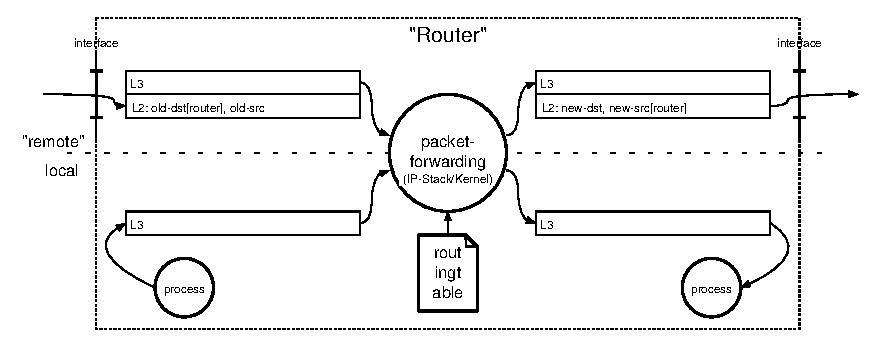
\includegraphics[width=16cm]{routing-packetforwarding}
\end{frame}

\begin{frame}
\frametitle{Routing: statisches Routing}
\begin{itemize}
  \item f\"ur kleine Netzwerke gen\"ugt statisches Routing:
    \begin{itemize}
      \item stub-net: nur ein Netzwerk und ein Router mit Verbindung zum ``Rest'' der Welt vorhanden\footnote{das ist genau die Konfiguration bei Ihnen zuhause}
      \item statische Netze mit wenigen Verbindungen dazwischen -- z.B. Firma mit Aussenstandorten \"uber Mietleitungen
    \end{itemize}
  \item dabei werden die Routing-Tabellen auf den beteiligten Ger\"aten manuell nachgef\"uhrt
  \item es k\"onnen ``alternative'' Wege eingetragen werden, die Routingtabelle bleibt aber statisch
\end{itemize}
\end{frame}


\begin{frame}
\frametitle{Routing: Stub-Network (statisch)}
\begin{center}
\includegraphics[width=10cm]{network-types-stub}
\end{center}
\end{frame}


\begin{frame}
\frametitle{Routing: Dynamisches Routing}
\begin{itemize}
	\item{automatische/dynamische Adaption bietet sich an bei:\begin{small}
	    \begin{itemize}
	       \item{grossen Netzwerken mit vielen Routern bei denen manuelle Anpassung der RT fehleranf\"allig/m\"uhsam w\"are}
	       \item{sich dynamisch ver\"andernden Netzwerken}
      \end{itemize}\end{small}}
  \item{dies wird durch {\em anpassen der Routing-Tabelle} aufgrund von {\em Topologie-Informationen} erreicht}
  \item{ein {\em Routing-Protokolle} (RP) hat die Aufgaben:\begin{small}
	    \begin{itemize}
	       \item{mit ``peers'' (anderen Routern) zu kommunizieren und Topologie-Informationen auszutauschen}
	       \item{die Routing-Tabelle entsprechend anpassen}
	       \item{\textbf{das Routing-Protokoll macht selber kein forwarding!}}
      \end{itemize}\end{small}}
\end{itemize}
\begin{block}{Dynamisches Routing}
Anpassen der Routing-Tabelle aufgrund von Topologie-Informationen.

Dynamisches Routing wird durch ``normale'' Prozesse/Programme mit Socket-Kommunikation erreicht
\end{block}
\end{frame}


\begin{frame}
\frametitle{Routing: Well-Connected-Network(s) {\small (dynamisch ist angesagt!)}}
\begin{center}
\includegraphics[width=10cm]{network-types-wellconnected}
\end{center}
\end{frame}



\begin{frame}
\end{frame}




\begin{frame}
\frametitle{Routing: RP$\leftrightarrow$RT Interaktion}
	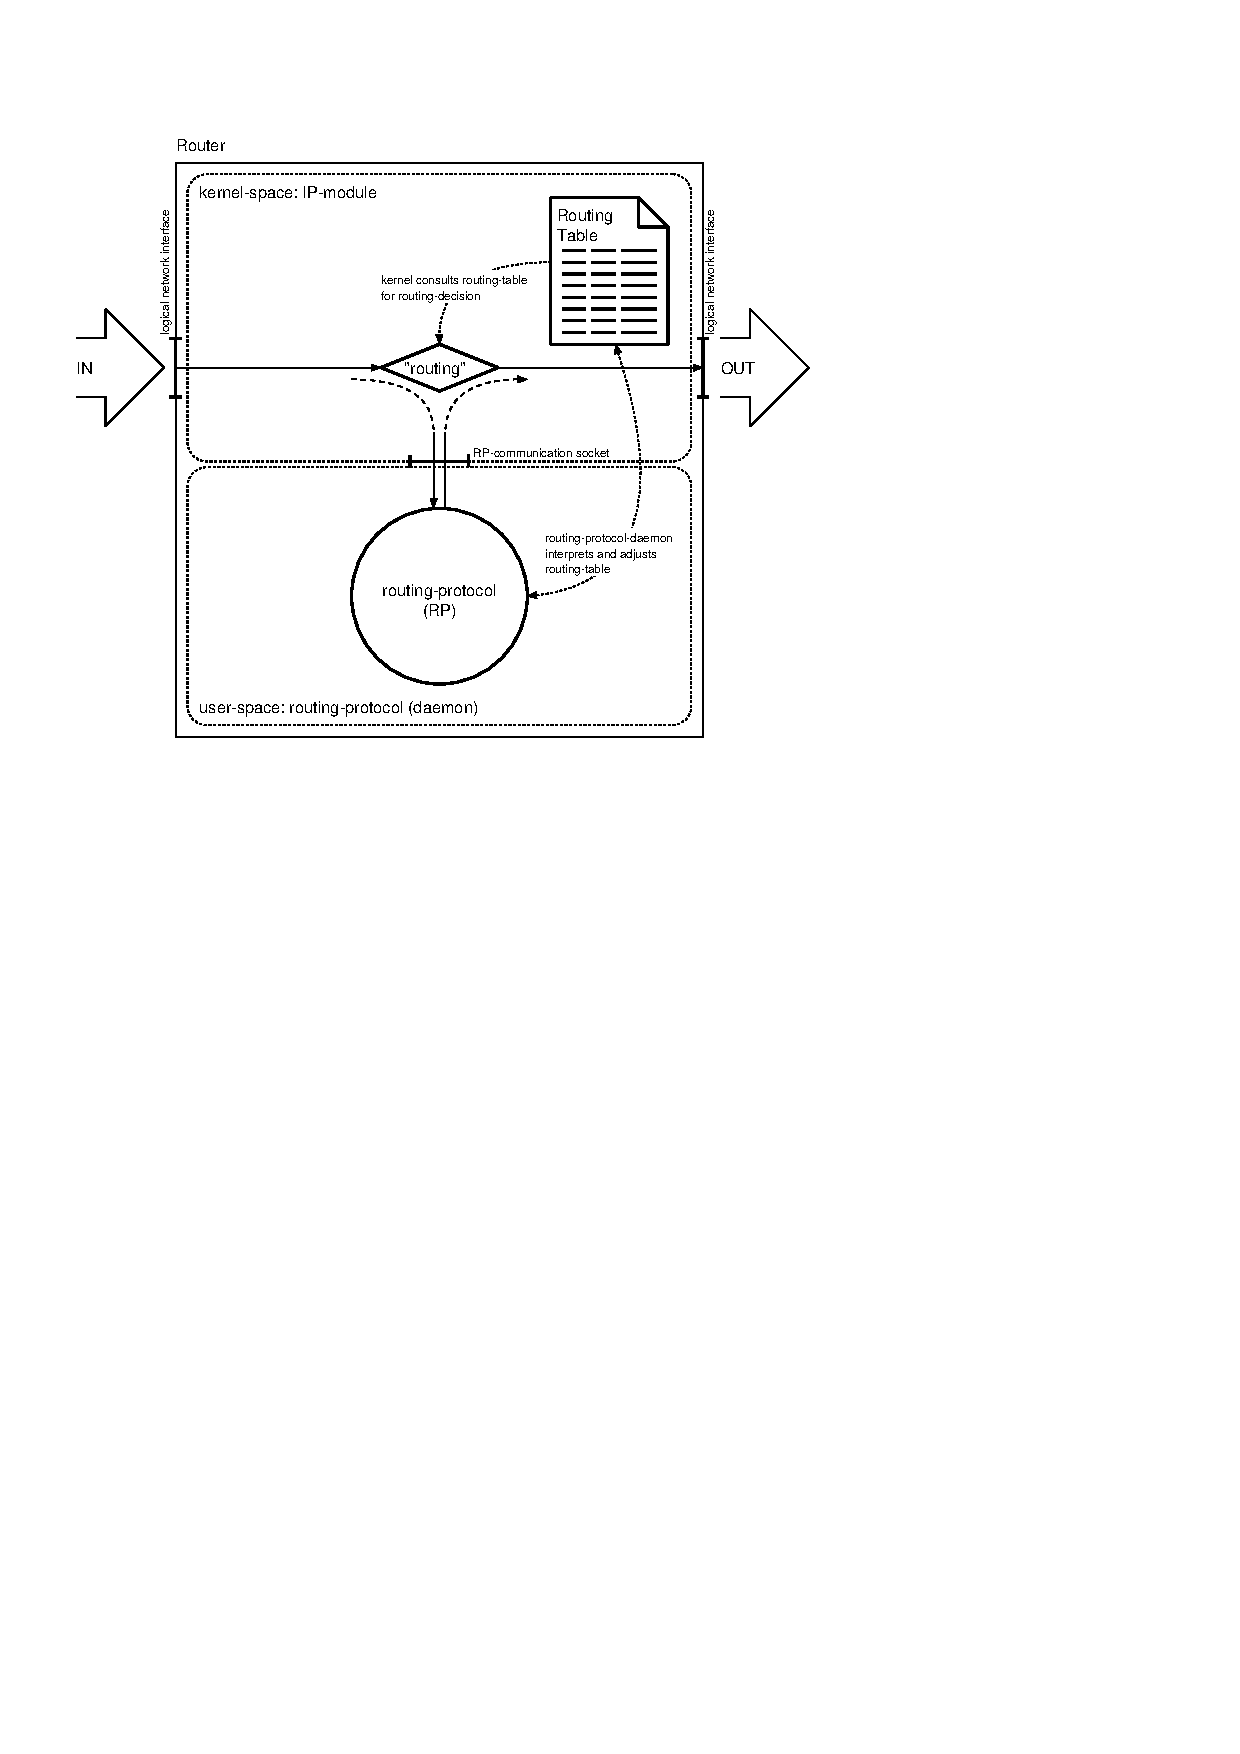
\includegraphics[height=19cm]{routing-detail}
\end{frame}


\begin{frame}
\frametitle{Routing: RT Updates}
Die Routing-Tabelle kann auf folgende Weise manipuliert werden:
\begin{itemize}
	\item{manuell durch editieren der RT (``statisches Routing``)}
	\item{durch ein Routing-Protokoll (``dynamisches Routing''}
	\item{durch \texttt{ICMP-REDIRECT}-Meldungen (``redirects'')}
\end{itemize}
\begin{center}
	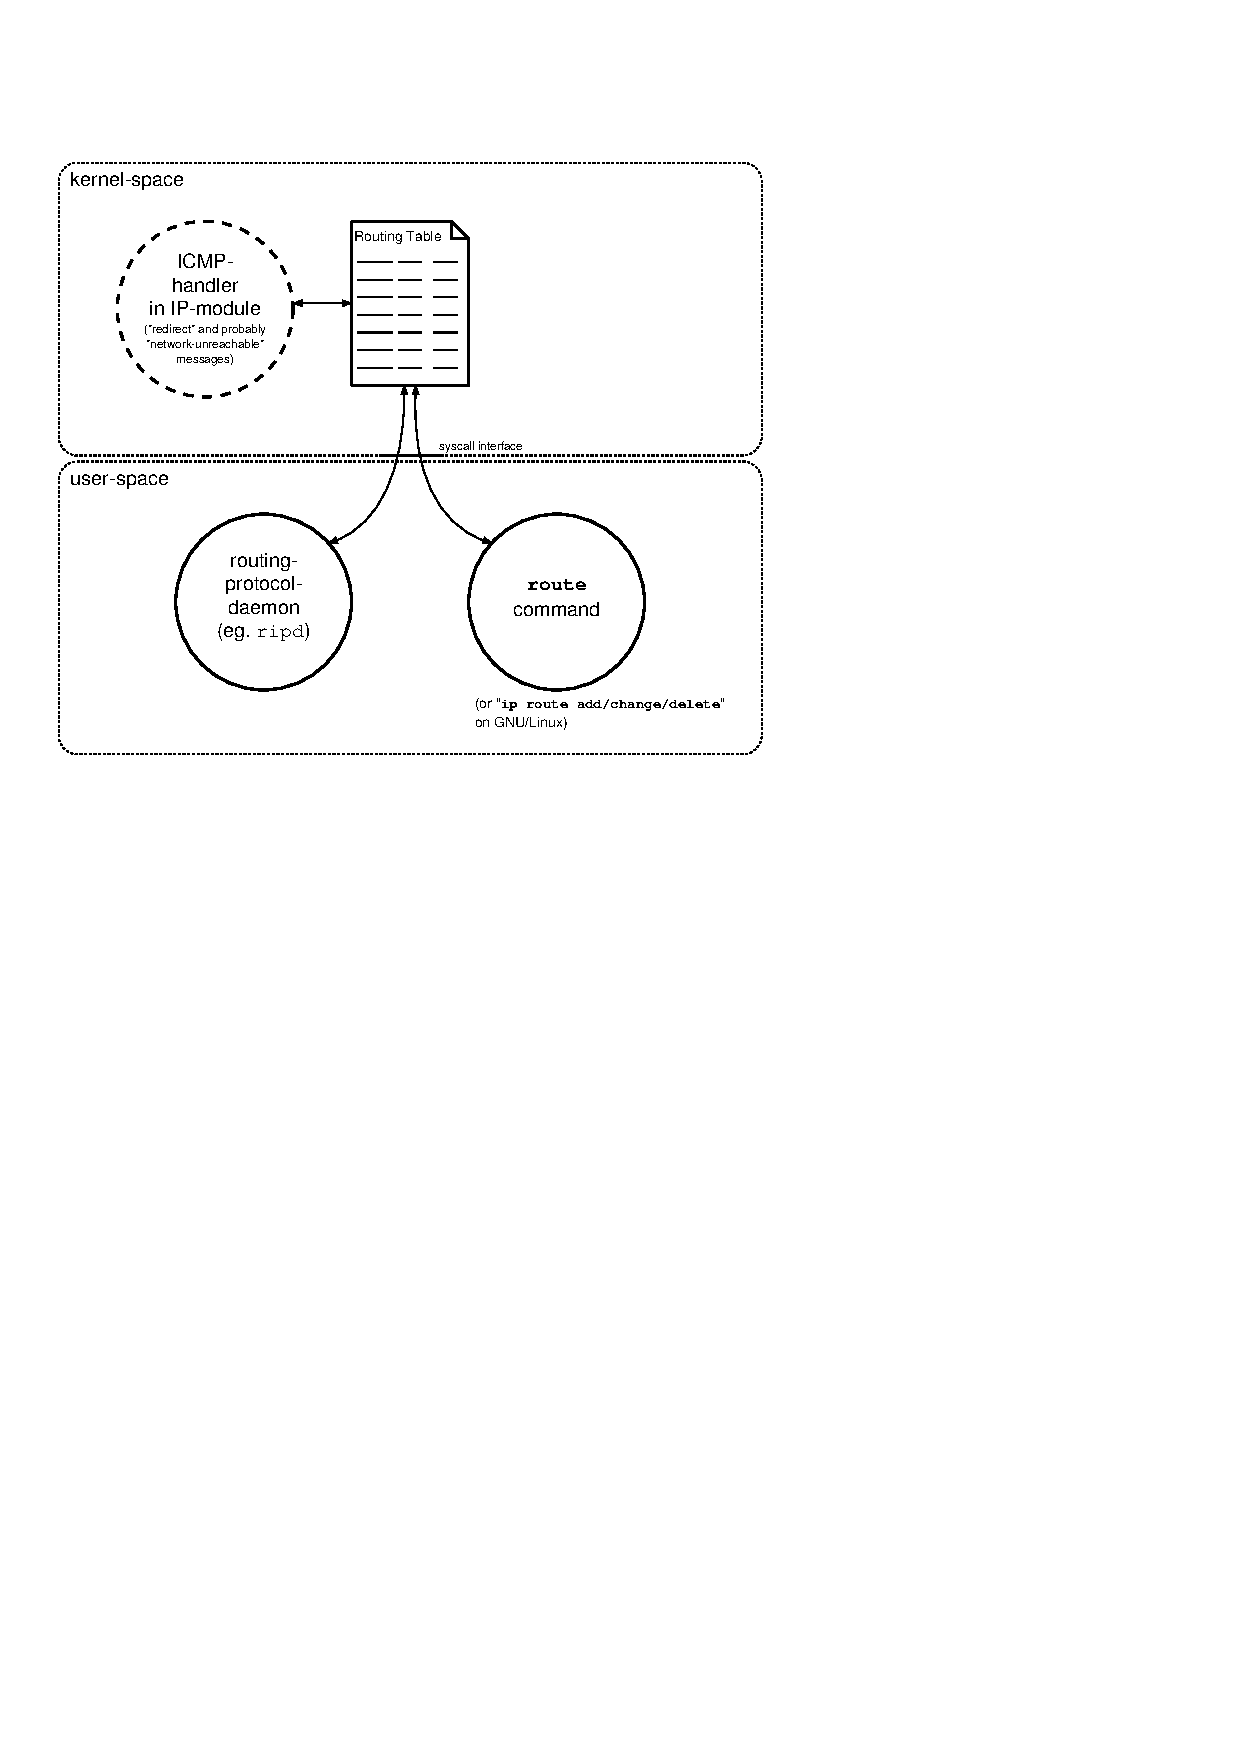
\includegraphics[height=14cm]{routing-rt-manipulation}
\end{center}
\end{frame}



\begin{frame}
\frametitle{Routing: Routing/Forwarding und Routing-Protokoll}
ein Host kann in Bezug auf ``Routing''folgende Rollen einnehmen:
\begin{itemize}
	\item{kein forwarding, kein routing-protocol: normales Endger\"at\footnote{Client oder Server}}
	\item{forwarding, kein routing-protocol: statischer Router}
	\item{kein forwarding, routing-protocol aktiv: ``Route Reflector'' oder ``Route Server''}
	\item{forwarding und routing-protocol: dynamischer Router}
\end{itemize}
\begin{center}
\includegraphics[width=6cm]{router-classification}
\end{center}
\end{frame}


\begin{frame}
\frametitle{Routing: Interior und Exterior Routing}
die Anforderungen an ein Routing-Protokoll unterscheiden sich je nach Anwendungszweck:
\begin{itemize}
	\item{\textbf{Interior Routing Protocol}: innerhalb einer Organisation\footnote{Hochschule, Firma, Service-Provider, etc}/\textbf{AS}\footnote{``autonomous system''} soll das Routing-Protokoll:\begin{small}
	    \begin{itemize}
	       \item{sich schnell an neue Situation anpassen (``konvergiert schnell'')}
	       \item{effizient arbeiten (nicht zuviele Daten senden/empfangen)}
	       \item{den {\em besten/schnellsten} Weg finden}
	       \item{m\"oglichst konfigurationslos arbeiten (``automatisch'')}
      \end{itemize}\end{small}}
	\item{\textbf{Exterior Routing Protocol}: {\em zwischen} Organisation, resp ``im Internet'' soll das Routing-Protokoll:\begin{small}
	    \begin{itemize}
	       \item{nicht-technische, d.h. ``politische'' Entscheidungen verwalten (``wer darf mit wem'', transit, etc)}
	       \item{Langzeitstabil sein (d.h. keine schnelle Oszillation ``route-flapping'')}
      \end{itemize}\end{small}}
\end{itemize}
Unabh\"angig davon sollte ein Routing-Protokoll:
\begin{itemize}
	\item{``loop-free'' arbeiten, d.h. keine Routing-Schlaufen generieren}
\end{itemize}
\end{frame}





\begin{frame}
\frametitle{Routing: Protokoll Familien}
Es wird im Allgemeinen zwischen drei Ans\"atzen unterschieden:
\begin{description}
	\item[Distance Vector] z.B. RIP{ \begin{tiny}
	  \begin{description}
	  	  \item[]
	    \item[information element\footnote{``was wird ausgetauscht''}:] Listen \texttt{\{network, metric\}} -- d.i. eine abgek\"urzte Routing-Tabelle
	    \item[communication peers\footnote{``mit wem kommuniziert das Routing-Protokoll''}:] mit allen direkten Nachbar-Router
			\item[topology inference\footnote{``wie wird die Netztopologie bestimmt''}:] aufgrund vorverarbeiteten Information\footnote{Sicht dieses Routers vom Netzwerk} von anderen Routern (summary, ``routing by rumors'')
	  \end{description}
	  \end{tiny}}
	\item[Link State] z.B. OSPF{ \begin{tiny}
	  \begin{description}
	  	  \item[]
	    \item[information element:] Listen \texttt{\{link/interface, state, metric\}} -- d.i. eine Liste der {\em Netzwerk-Interfaces} und ihr Zustand (up, down)
	    \item[communication peers:] mit {\em allen Routern im Netzwerk}
			\item[topology inference:] aufgrund gesicherten {\em lokalen Informationen} der Router
	  \end{description}
	  \end{tiny}}
	\item[Path Vector] z.B. BGP{ \begin{tiny}
	  \begin{description}
	  	  \item[]
	    \item[information element:] komplexe Listen \texttt{\{net, path-element$_{1}$, path-element$_{2}$, ..., other-attributes*\}} -- d.i {\em Pfad} zum Ziel
	    \item[communication peers:] mit ausgew\"ahlten {\em Peer-Routern} (peering)
			\item[topology inference:] magisch
	  \end{description}
	  \end{tiny}}
\end{description}
\end{frame}





\begin{frame}
\frametitle{Routing: Distance Vector am Beispiel von RIP}
Das {\bf R}outing {\bf I}nformation {\bf P}rotocol\footnote{nein, nicht ``Rest In Peace'', wobei das in diesem Fall angebracht w\"are} ist ein lebendes Fossil aus der IP-Steinzeit:
\begin{description}
	\item[Information Element]: distance vector --- a list of
		{\tt \{network, distance\}} tuples. Distance is measured in
		count of ``hops'' to reach a network; one hop being a router
	\item[Communication Peers]: broadcast on all connected networks, UDP 520
	\item[Topology Inference]: (none), distributed Bellman-Ford algorithm\footnote{RIP
		is based on the fact that only the next-hop
		to a certain destination must be known for correct routing-operation. A single
		RIP-instance is not able to determine the real network topology}
	\item[Operation]: RIPv1 sends DV-elements in fixed intervals to the broadcast
		addresses of all connected networks (interfaces):
		\begin{tiny}
		\begin{itemize}
			\item send own routing-table (only network w/o mask and hop-count metric) broadcast
			\item received DVs are compared element-wise with the existing
				routing-table; entries with minimal metric are kept, all other
				information is dropped
			\item every (dynamically learned) routing-table entry will eventually
				time-out if it is not updated by new received DV
		\end{itemize}
		\end{tiny}
	\item[Pros]: ubiquitous (everyone talks and understands RIP)
	\item[Cons]: (too many, see next slide)
\end{description}
\end{frame}

\begin{frame}
\frametitle{Routing: Notation Beispiele}
\begin{center}
\includegraphics[height=8cm]{simplified-view}
\end{center}
\end{frame}



\begin{frame}
\frametitle{Routing: RIP Beispiel}
\begin{center}
\includegraphics[width=12cm]{rip-network}
\end{center}
\end{frame}



\begin{frame}
\frametitle{Routing: RIP Beispiel, Step 1}
\begin{center}
\includegraphics[width=12cm]{rip-step-1}
\end{center}
\end{frame}



\begin{frame}
\frametitle{Routing: RIP Beispiel, Step 2}
\begin{center}
\includegraphics[width=12cm]{rip-step-2}
\end{center}
\end{frame}



\begin{frame}
\frametitle{Routing: RIP Tabellen}
\begin{center}
\includegraphics[width=12cm]{rip-table}
\end{center}

\end{frame}

\begin{frame}
\frametitle{Routing: RIP Nachteile}
\begin{itemize}
	\item ``routing by rumors''
	\item too simple metric
	\item limited diameter (max 15 hops)
	\item classful behavior (implicit class-netmask)
	\item slow convergence; fixed intervals and flawed method
	\item loops/gaps; ``counting to infinity'', etc
	\item no authentication
	\item traffic grows uncanny for bigger networks
	\item broadcast communication
\end{itemize}
\end{frame}



\begin{frame}
\frametitle{Routing: RIPv2 Fixes}
\begin{description}
	\item[metric]: tweak ``interface cost'' such that slower links will count
		more than one host\footnote{eg {\tt man ifconfig}}
	\item[classful behavior]: RIPv2 solves this problem: DV contains {\tt 		(network,mask,distance)} tuples
	\item[slow convergence]: ``triggered updates'', event-driven DV-broadcast. Implemented
		as an option to RIPv1 and mandatory in RIPv2
	\item[loops/gaps]: ``split horizon'' and ``poisoned reverse''. Implemented as an option
		to RIPv2, mandatory in RIPv2
	\item[authentication]: implemented in RIPv2
	\item[broadcast communication]: RIPv2 supports multicast instead of broadcast
\end{description}
\begin{tiny}
RIPv2 still suffers from ``routing by rumors'', ``simple metric'' (although there is support for
additional metrics), ``limited diameter'' and ``traffic growth''. Besides this, RIPv2/RIPv1
coexistence is not as seamless as it may be: why not just a real routing-protocol\texttrademark?
\end{tiny}
\end{frame}




\begin{frame}
\frametitle{Routing: Link State am Beispiel von OSPF}
{\em O}pen {\em S}hortest {\em P}ath {\em F}irst is
capable of handling even the largest corporate networks\footnote{we
are talking about {\em interior routing} here... The Internet
would be happy with OSPF too -- if not for the politics... (see slide \pageref{BGP})}
\begin{small}
\begin{description}
	\item[Information Element:] LSA, the {\em L}ink {\em S}tate {\em A}dvertisment.\\A List
		of tuples {\tt (link, state, metric...)}\footnote{the combined length of all LSAs
		in a network grows sub-polynomial, the length of a single LSA only changes
		if links where added or removed --- compare this situation to RIP}
	\item[Communication Peers:] Communication in OSPF if twofold:\begin{tiny}
		\begin{itemize}
			\item HELLO-protocol to discover and check reachability of neighbours
			\item LSA distribution through a {\em flooding} mechanism to all OSPF-routers in the network
		\end{itemize}\end{tiny}
	\item[Topology Inference:] Djikstra's spanning tree algorithm --- full topology available
		from LSDB\footnote{extended adjacency matrix determined by combining all received LSAs}
	\item[Operation:] \begin{tiny}
		\begin{description}
			\item[neighbor/link integrity:] through periodic HELLO-packet to neighbor routers {\tiny very
				short packets, interval adjustable (common values 5, 10, 30 seconds)}
			\item[flooding LSA:] on start-up or changes to interface/link-state, a LSA-packet is \emph{flooded}
				to the entire OSPF-network (area)
			\item[RT-calculation:] by Djikstra's algorithm
		\end{description}\end{tiny}
	\item[Pros:] (too many, see next slide)
	\item[Cons:] CPU- and memory-load may be a concern if used on {\em old crappy} hardware
\end{description}
\end{small}
\end{frame}



\begin{frame}
\frametitle{Routing:Link-State Djikstra (1/3)}
\vspace{1cm}
	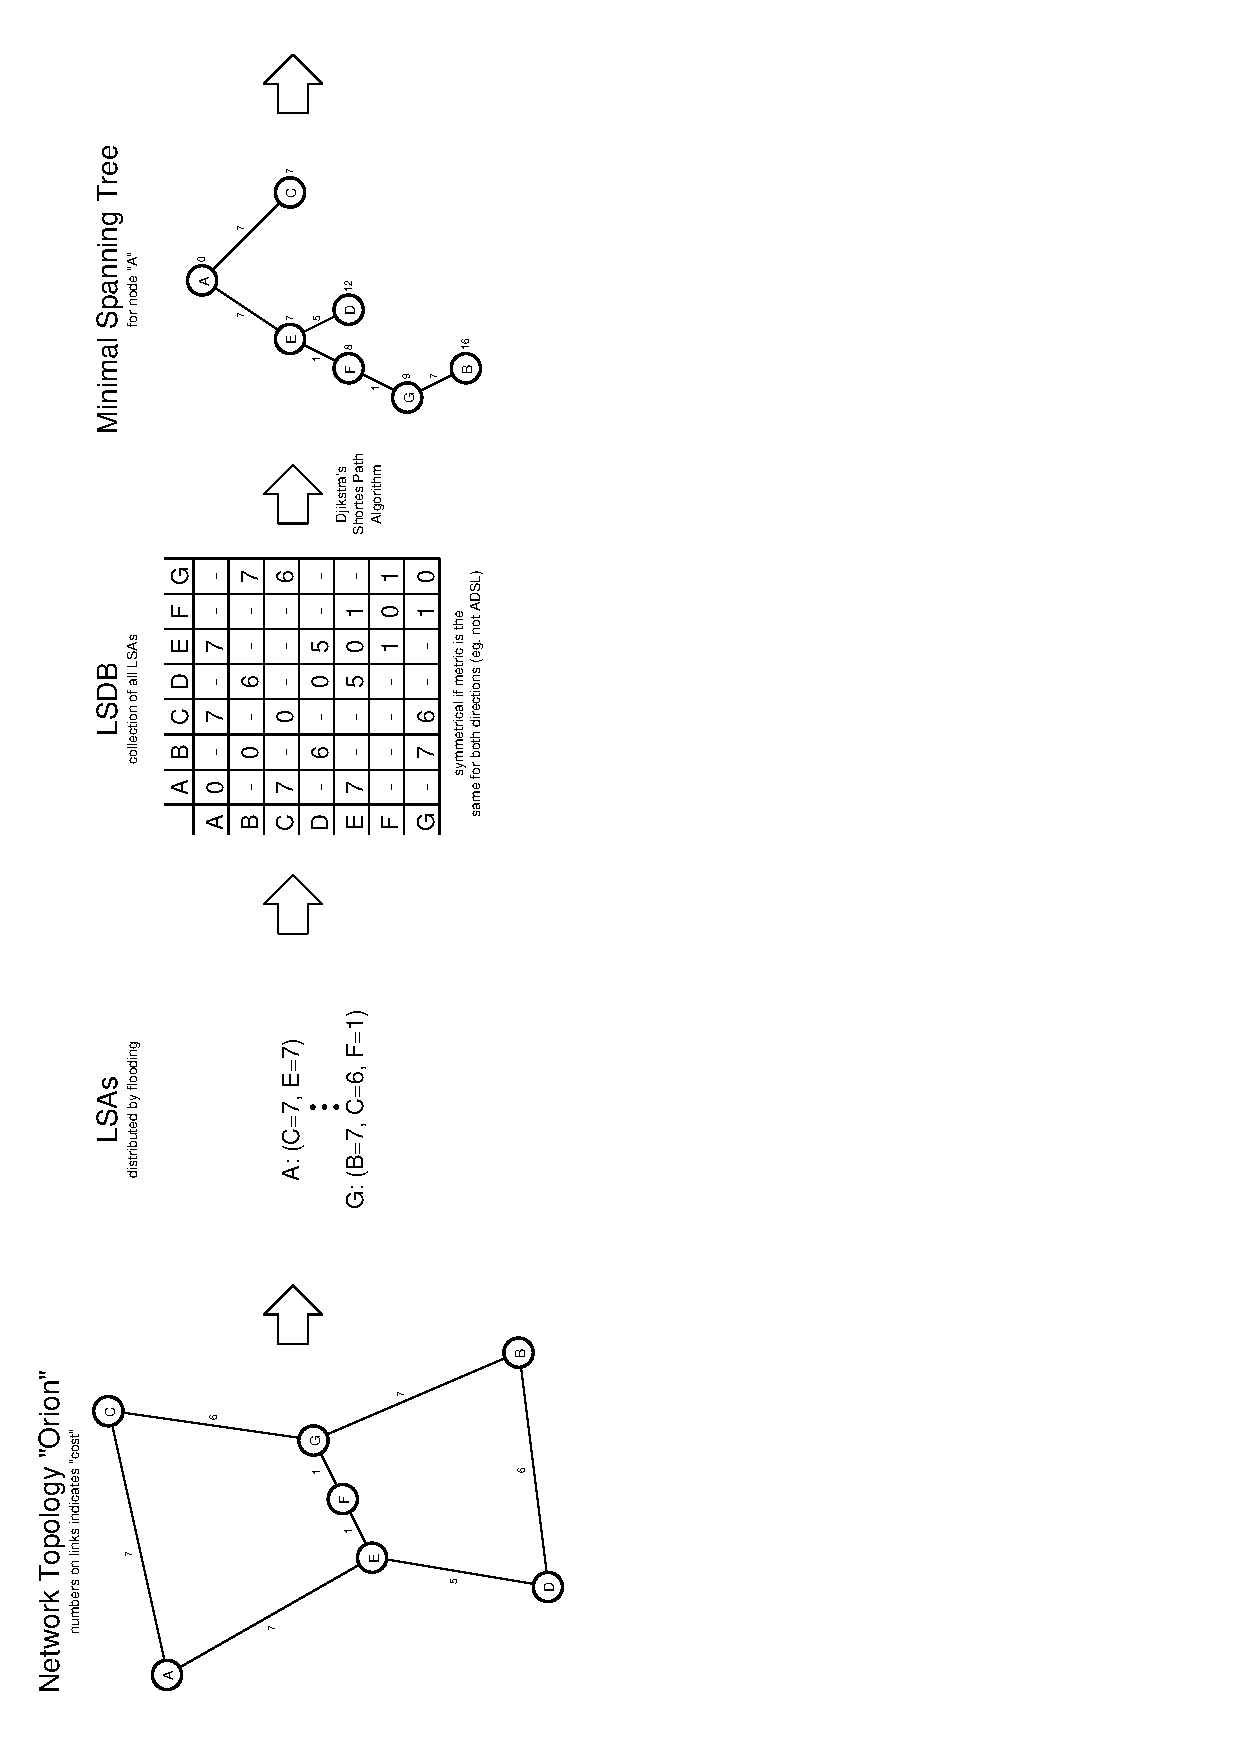
\includegraphics[height=9cm]{orion-cost}
\end{frame}


\begin{frame}
\frametitle{Routing: Link-State Djikstra (2/3)}
``a not-so-formal description of Djikstras Spanning-Tree-Algorithm''
\begin{tiny}
\begin{tabular}{|p{3cm}|p{4cm}|p{4cm}|}
\hline
{\bf Initialization} & {\bf Loop} & {\bf Result} \\
\hline
\hline
\begin{minipage}[t]{3cm}
	\begin{tabbing}
		\hspace{0.5cm}\=\hspace{0.5cm}\=\kill
		c \>$\leftarrow$ selected-root-node\\
		{\bf A} \>$\leftarrow$ \{ c \}\\
		{\bf F} \>$\leftarrow$ \{ all-nodes \} $\setminus$ c\\
		{\bf T} \>$\leftarrow$ \{\}\\
	\end{tabbing}
\end{minipage} &
\begin{minipage}[t]{4cm}
	\begin{tabbing}
		\hspace{0.5cm}\=\hspace{0.5cm}\=\hspace{0.5cm}\=\hspace{0.5cm}\=\kill
		while {\bf F} $\neq$ \{\} do\\
		\> for each neighbor n of c still in {\bf F} do\\
		\>\> if n $\exists$ {\bf T}\\
		\>\>\> if cost(n) $<$ cost(n $\in$ {\bf T})\\
		\>\>\>\> {\bf T} $\leftarrow$ {\bf T} - (n $\in$ {\bf T}) + n\\
		\>\>\> else\\
		\>\>\>\> {\bf T} $\leftarrow$ {\bf T} + n\\
		\>\>\> end-if\\
		\>\> else \\
		\>\>\> {\bf T} $\leftarrow$ {\bf T} + n\\
		\>\> end-if\\
		\> end-for\\
		\>set c to minimum cost node from {\bf T}\\
		\> {\bf A} $\leftarrow$ {\bf A} + c\footnotemark\\
		\> {\bf T} $\leftarrow$ {\bf T} $\setminus$ c\\
		\> {\bf F} $\leftarrow$ {\bf F} $\setminus$ c\\
		end-while
	\end{tabbing}
\end{minipage} &
\begin{minipage}[t]{4cm}
	\begin{tabbing}
		\hspace{0.5cm}\=\hspace{0.5cm}\=\kill
		{\bf F} \>= \{\}\\
		{\bf A} \>= \{ topologically sorted list \}\\
	\end{tabbing}
\end{minipage} \\
\hline
\end{tabular}
\footnotetext{this involves also adding it permanently to the tree... ie: add new c as a child of former c}
\end{tiny}
\end{frame}

\begin{frame}
\frametitle{Routing:Link-State Djikstra (3/3)}
\vspace{1cm}
	
\includegraphics[height=4cm]{djikstra-tree-0}
	\includegraphics[height=4cm]{djikstra-tree-1}
	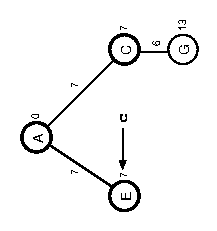
\includegraphics[height=4cm]{djikstra-tree-2}
	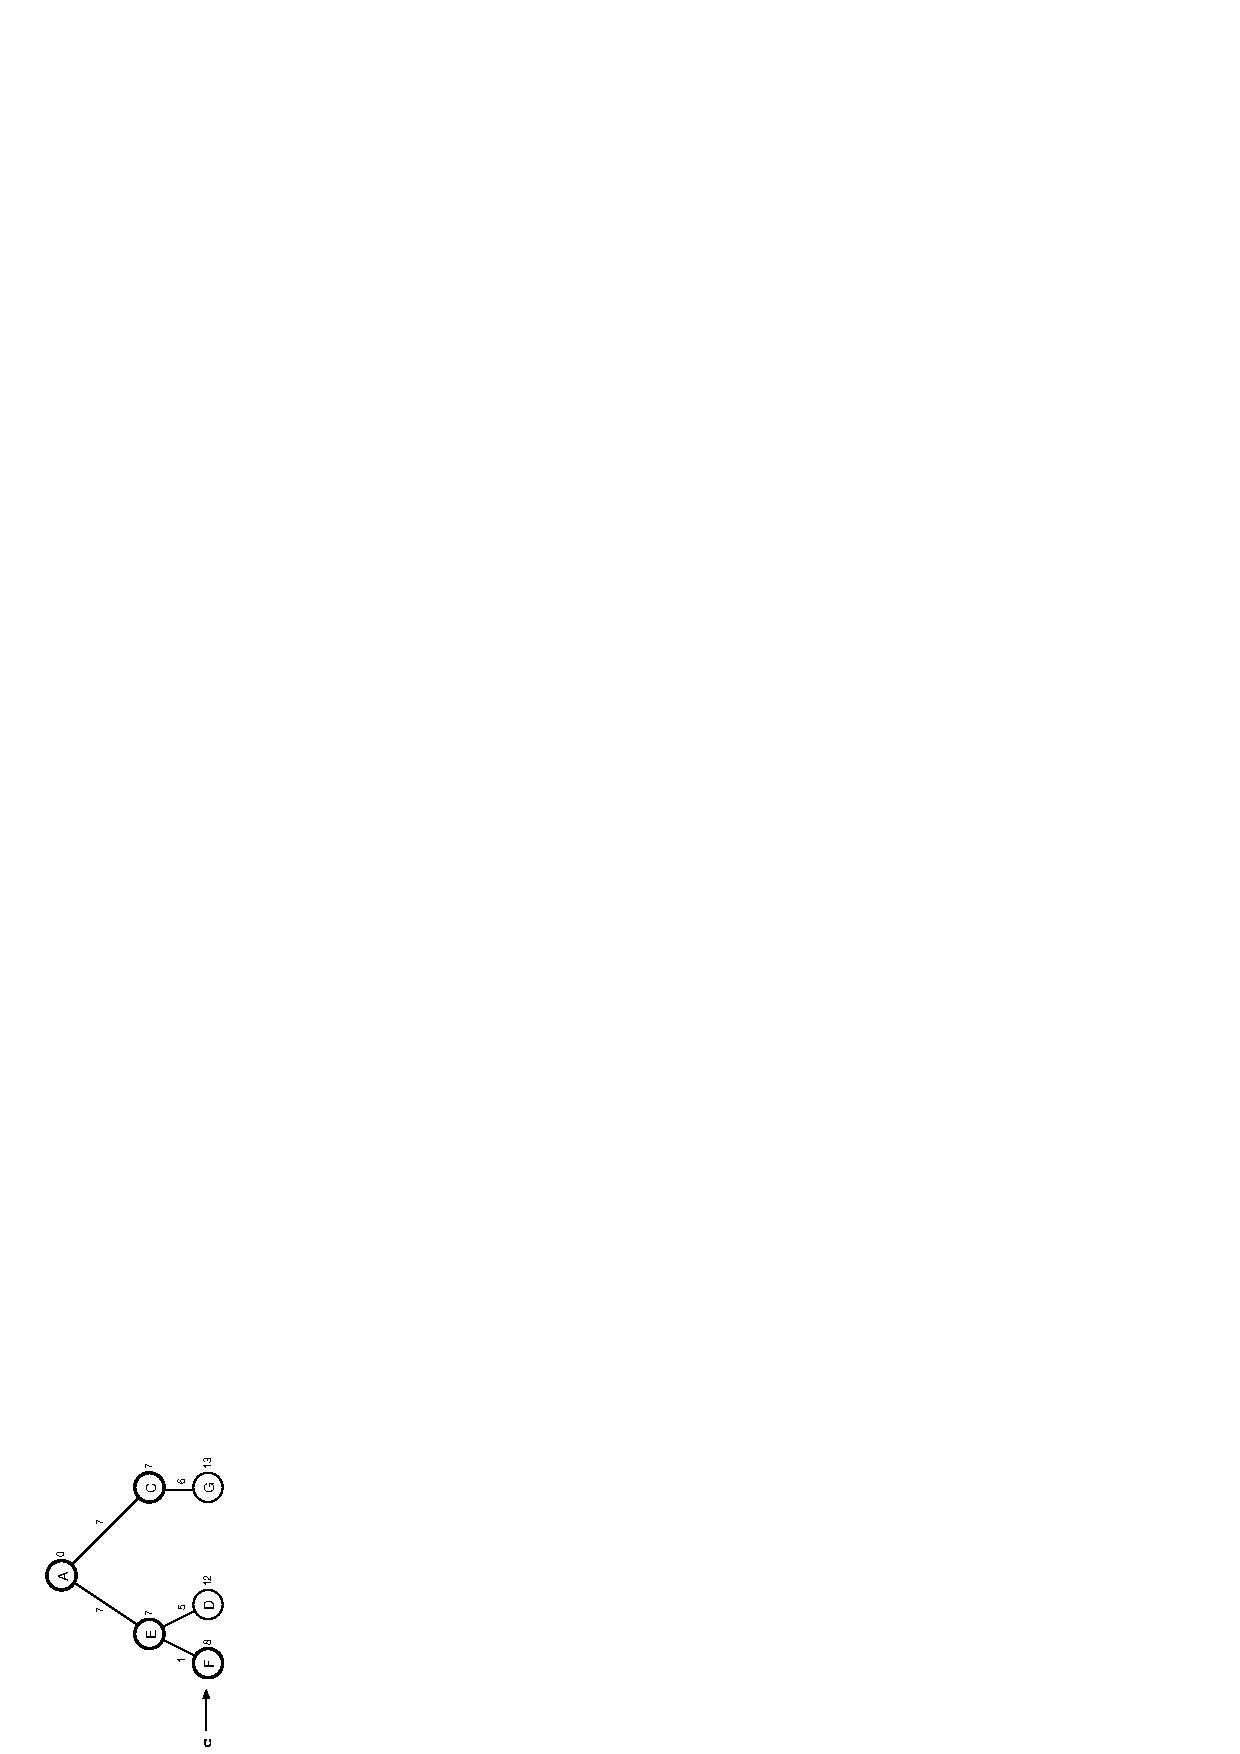
\includegraphics[height=4cm]{djikstra-tree-3}
\\
\vspace{-1cm}

	\includegraphics[height=4cm]{djikstra-tree-4}
	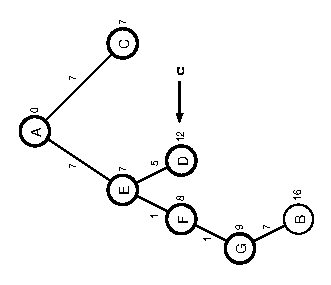
\includegraphics[height=4cm]{djikstra-tree-5}
	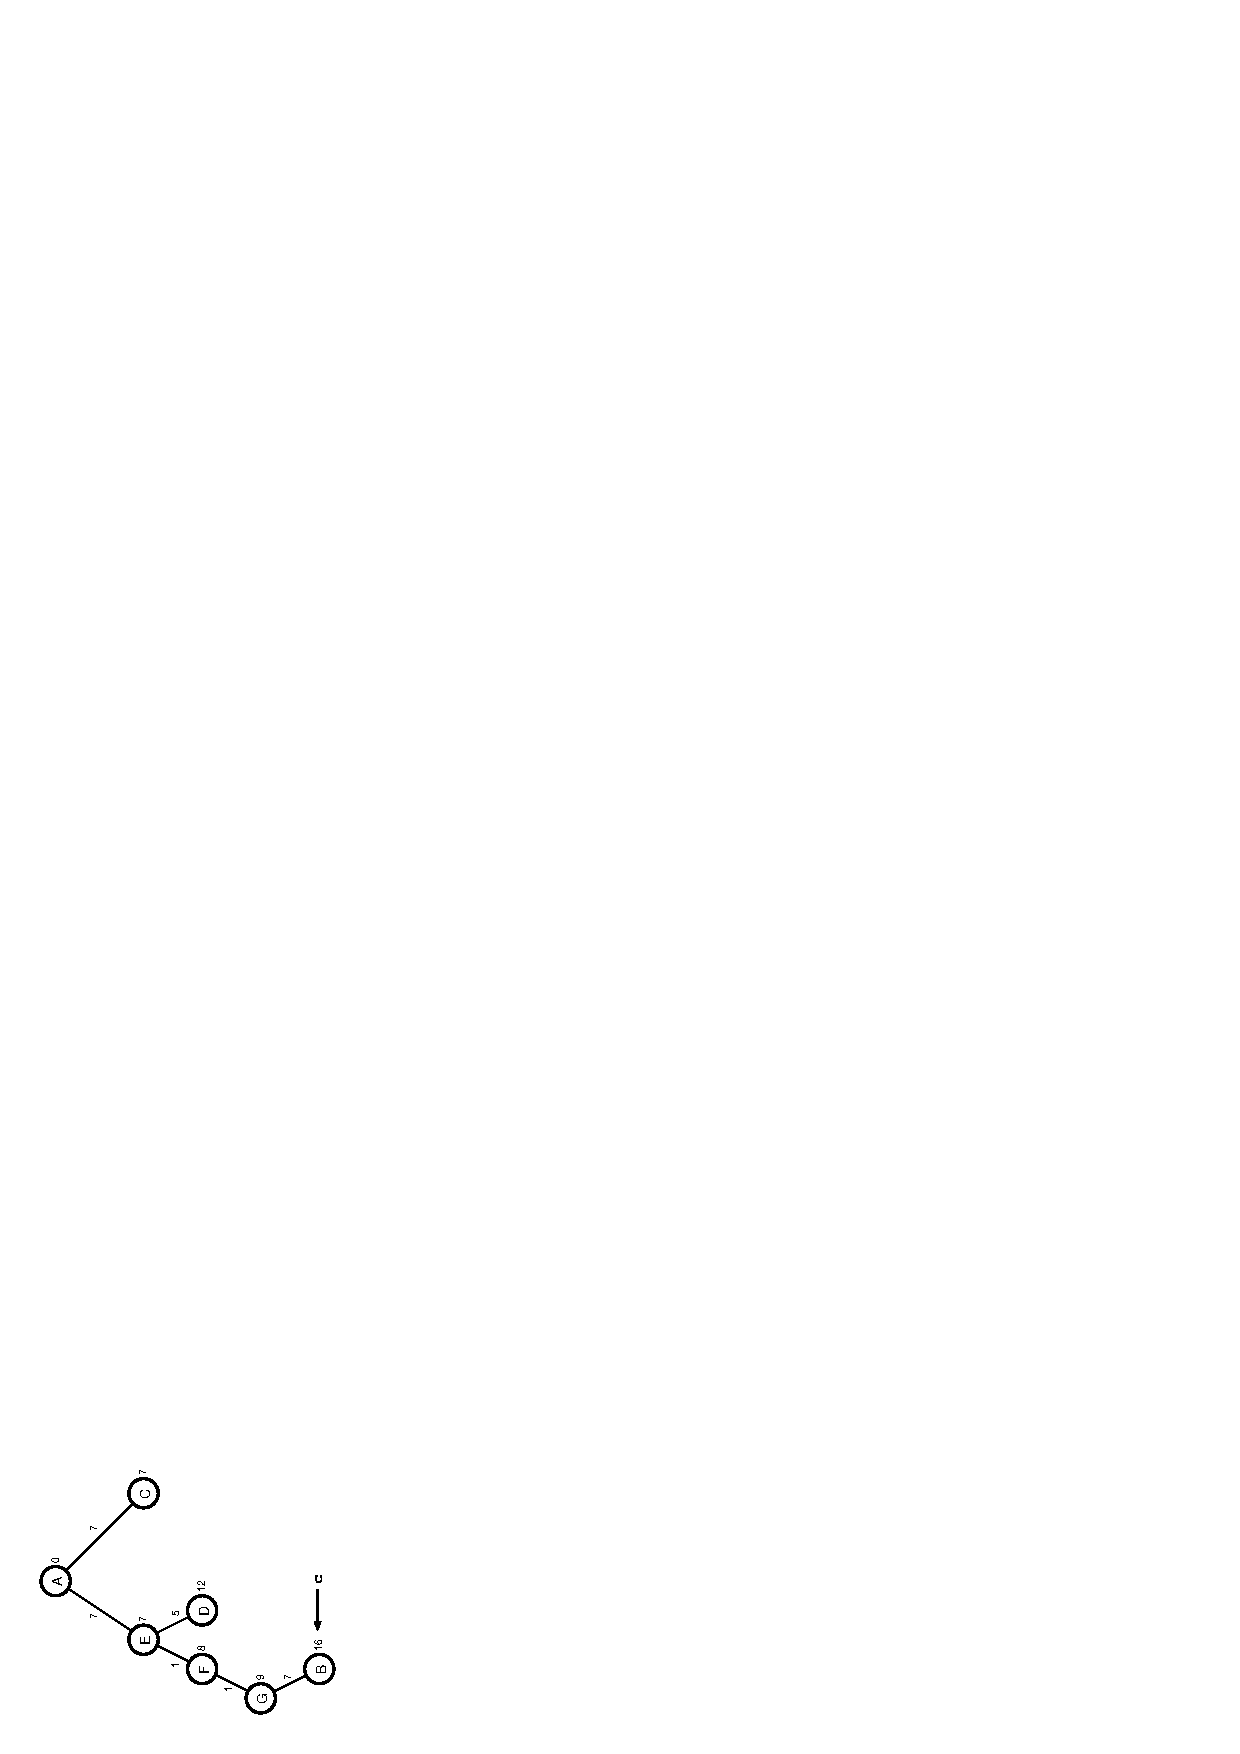
\includegraphics[height=4cm]{djikstra-tree-6}
\end{frame}



\begin{frame}
\frametitle{Routing: OSPF Vorteile}
\begin{description}
	\item[Djikstra] Schleifen-freie Topologie-Ableitung (``spanning-tree'')
	\item[Areas] Unterteilung in Teilgebiete, z.B. ``Backbone'' und ``Site'' mit Delegation
	\item[Virtual Links] nicht-physikalische Verbindungen k\"onnen abgebildet werden
	\item[Multicast] es werden nur OSPF-Router angesprochen (vergl. RIPv1 broadcast)
	\item[Aggregating] ein Teilgebiet kann als ``kleines AS'' (blackbox) zusammengefasst werden
	\item[Security] authenticated messages, viel schwieriger anzugreifen als RIP
\end{description}
\end{frame}






\begin{frame}
\frametitle{Routing: Path Vector}
\vfill
\centerline{and now for something completely different$\ldots$}
\end{frame}


\begin{frame}
\label{BGP}
\frametitle{Routing: Internet ``AS-jungle''}
\begin{small}
Routing in the Internet is based on ``autonomous systems'' (AS), regarded as black boxes, 
ie the \emph{AS-internal} routing procedure is hidden at the AS-border
\hspace{-0.5cm}
\begin{minipage}[t]{3.5cm}
	\begin{tiny}
	\begin{itemize}
		\item ASes are usually ISPs or large corporations with redundant connections to the Internet (\emph{multi-homed})
		\item AS-numbers are allocated globally\footnotemark[21], ie this are unique identifiers
		\item ISPs usually gather together at ``Internet Exchange'' points\footnotemark[22], a physical
			location to form a star-network topology
		\item BGP is used between ASes to exchange routing-information \emph{based on AS structures}
			(ie, large-scale routing)
		\item BGP allows to perform \emph{policy based routing} (ie, not only based on destination)
	\end{itemize}
	\end{tiny}
\end{minipage}
\footnotetext[21]{today the numbers are allocated from the continental-blocks from ARIN, RIPE, APNIC}
\footnotetext[22]{IX, NAPs, [Mega]POPs. Eg, CernCIX and Telehouse Zurich TIX in Switzerland}
\end{small}
\begin{minipage}[t]{8cm}
	\hspace{-1cm}\vspace{-0.5cm}
	\begin{center}
		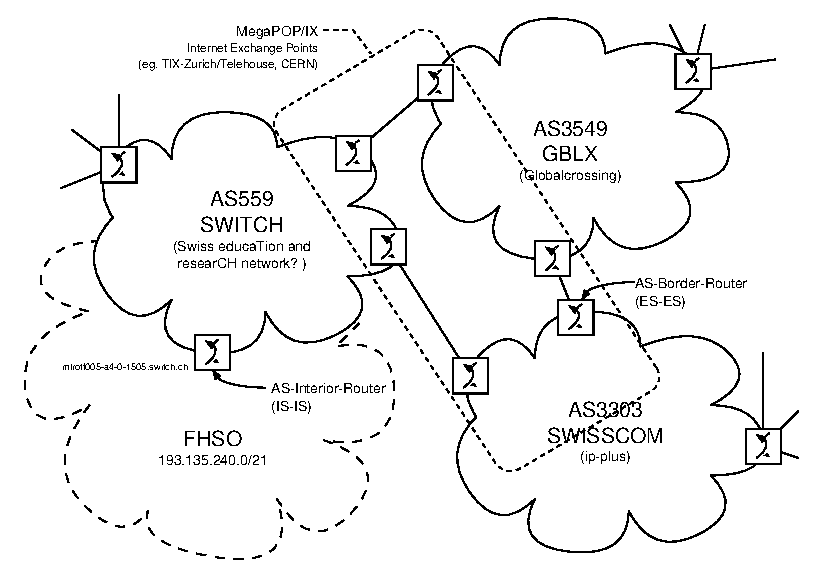
\includegraphics[width=12cm]{routing-as}
	\end{center}
\end{minipage}
\end{frame}



\begin{frame}
\frametitle{Routing: BGP-Announcements}
\begin{center}
	\includegraphics[width=12cm]{routing-bgp-updates}
\end{center}
\end{frame}







\begin{frame}[fragile]
\frametitle{Routing: BGP}
Dynamic routing in the Internet is done by
the {\bf B}order {\bf G}ateway {\bf P}rotocol
\begin{description}
	\item[Information Element]: path-vector, a prefix\footnote{ie, IP/prefixlength} and a list
		of ASes (in-reverse) to reach it

		\begin{tiny}
			an actual example (edited) from AT\&T=AS7018 (query is part of Solnet=AS9044):
			\begin{verbatim}
BGP routing table entry for 212.101.0.0/19:
  7018 3549 9044 9044, (received & used)
			\end{verbatim}
			read: to reach 212.101.0.0/19 from AT\&T, the packet must pass through
			AT\&T (AS7018), Global Crossing (GBLX, AS3549) and finally Solnet (AS9044)
		\end{tiny}
	\item[Communication Peers]: strictly point-to-point using TCP port 179. The connections
		must be configured manually (UDP 179 only for I-BGP)
	\item[Topology Inference]: this is remains a miracle
	\item[Operation]: 
		\begin{tiny}
			\begin{itemize}
				\item OPEN connection to peer
				\item send NOTIFICATION in case of errors or to close the session
				\item send KEEPALIVE periodically (60 seconds beeing reasonable, hold-up is usually set to
					three times keepalive)
				\item send UPDATE as: ``{\tt prefix: \emph{MY-AS\#} [\emph{existing-AS-path}], NEXT-HOP=\emph{MY-IP}}'', ie \emph{prepend} the own AS\# to the path
				\item select best (shortest, policy-based, etc) path from the received UPDATES, generate RT
			\end{itemize}
		\end{tiny}
	\item[Pros]: there is no alternative
	\item[Cons]: there is no alternative
\end{description}
\end{frame}







\begin{frame}
\frametitle{Routing: BGP Factlets}
\begin{description}
	\item[Loop-Prevention:] loops are resolved by filtering the path for repetitious elements
	\item[Best-Path:] in absence of other criteria, the best path is the shortest\footnote{AS-wise, ie
		there is no possibility to infer the actual hop-count \emph{inside} one AS} one. Although
		BGP (the process) allows almost arbitrary filtering and mangling of attributes, thus very
		sophisticated selection of paths are possible
	\item[I-BGP, E-BGP:] large AS may run BGP AS-internal. This allows load-sharing and
		flexible adaption to AS-AS connection changes
\end{description}
\end{frame}







\begin{frame}[fragile]
\frametitle{Routing: BGP Informationen 1/2}
BGP ``politics'' Informationen kann mit \texttt{whois} oder \"uber eine geeignete Webseite gefunden werden\footnote{wenn sie nicht selbst ein AS verwalten, resp. ein BGP-peer sind. \myurl{http://www.ripe.net/} f\"ur Europa}
\begin{tiny}
Dabei wird der {\em AS-Path}{} zu einem Ziel angezeigt, d.h. nicht einzelne Router wie bei \texttt{traceroute} sondern AS (z.B. Internet Service Providers) als ``black box''
\end{tiny}
\begin{itemize}
	\item[radb:]{die routing arbiter database \myurl{http://www.ra.net/}, Beispiel (edited):
	  \begin{tiny}
	  \begin{verbatim}
rschmutz@callisto routing $ host www.post.ch
www.post.ch has address 194.41.161.1

# query RADB http://www.ra.net/ with 194.41.161.1

route:	      194.41.128.0/18
descr:	      CH-POST-040816
origin:	      AS12511

# query RADB http://www.ra.net/ with AS12511

aut-num:      AS12511
descr:        Die Schweizerische Post
import:       from AS6730
              action pref=100;
              accept ANY
import:       from AS3303
              action pref=100;
              accept ANY
export:       to AS6730
              announce AS12511
export:       to AS3303
              announce AS12511
	  \end{verbatim}
	  \end{tiny}
	}
\end{itemize}
\end{frame}






\begin{frame}[fragile]
\frametitle{Routing: BGP Informationen 2/2}
oder \"uber einen {\em Route-Server}{}\footnote{auch route-reflector. Liste bei \myurl{http://www.traceroute.org/\#Route\%20Servers}}:
\begin{itemize}
	\item[gblx]{
	  \begin{tiny}
	  \begin{verbatim}
telnet route-server.gblx.net
...
route-server.phx1>show ip bgp 194.41.161.1
BGP routing table entry for 194.41.128.0/18, version 39211644
Bestpath Modifiers: always-compare-med, deterministic-med
Paths: (1 available, best #1)
  Not advertised to any peer
  6730 12511 12511 12511 12511, (received & used)
    67.17.64.89 from 67.17.82.146 (67.17.82.146)
      Origin IGP, localpref 300, valid, internal, best
      Community: 3549:4723 3549:31756
      Originator: 67.17.80.142, Cluster list: 0.0.0.141
	  \end{verbatim}
	  \end{tiny}
	}
\end{itemize}
\end{frame}




\begin{frame}[fragile]
\frametitle{Routing: BGP Coole Tools}

\begin{itemize}
  \item ``Looking-Glass/LG'' Server sind Web-GUIs auf bekannte tools wie \texttt{traceroute}, \texttt{ping}, \texttt{show ip bgp}: \myurl{http://traceroute.org/\#Looking\%20Glass}, z.B. \myurl{https://lg.he.net/}
  \item RIPE\footnote{der Europ\"aische ``Regional Internet Registrar''} hat ein sehr cooles ``live'' BGP-Tool: \myurl{https://ris-live.ripe.net/}
  \item farbenfrohe Meta-Seite zu BGP: \myurl{https://www.bgp4.as/tools}
  \item RIPE hat ebenfalls eine Zusammenfassung von ``whois'' und Routing-Informationen: \myurl{https://stat.ripe.net/} -- dies klappt auch mit Netzwerken ausserhalb der RIPE-Registrierung

  \item mit einem lokalen \texttt{telnet} oder \texttt{nc/netcat/ncat}-Client k\"onnen auch interaktive Sessions auf ``echte'' Route-Server im Internet gemacht werden:
\begin{tiny}\verbatiminput{routing-he-route-server.txt}\end{tiny}

\end{itemize}
	
\end{frame}





\end{document}